%
% sesion7.tex
% 
% Copyright 2014 Rony J. Letona <zronyj@gmail.com>
% 
% This program is free software; you can redistribute it and/or modify
% it under the terms of the GNU General Public License as published by
% the Free Software Foundation; either version 2 of the License, or
% any later version.
% 
% This program is distributed in the hope that it will be useful,
% but WITHOUT ANY WARRANTY; without even the implied warranty of
% MERCHANTABILITY or FITNESS FOR A PARTICULAR PURPOSE.  See the
% GNU General Public License for more details.
% 
% You should have received a copy of the GNU General Public License
% along with this program; if not, write to the Free Software
% Foundation, Inc., 51 Franklin Street, Fifth Floor, Boston,
% MA 02110-1301, USA.
%

\documentclass[10pt,letterpaper]{article}
\usepackage[latin1]{inputenc}
\usepackage[spanish]{babel}
\usepackage{graphicx}
\usepackage{hyperref}
\usepackage{amsmath}
\usepackage{amsfonts}
\usepackage{amssymb}
\usepackage{color}
\usepackage{float}
\usepackage[left=2cm,right=2cm,top=2cm,bottom=2cm]{geometry}
\author{Rony J. Letona}
\title{Taller de Qu\'imica Computacional Aplicada: Sesi\'on 7}
\definecolor{light-gray}{gray}{0.90}

\newcommand{\tab}[1]{\hspace{.2\textwidth}\rlap{#1}}

\newcommand{\inlinecode}[1]{
\colorbox{light-gray}{\texttt{#1}}
}

\newsavebox{\selvestebox}
\newenvironment{Code}
{
\begin{lrbox}{\selvestebox}%
\begin{minipage}{\dimexpr\columnwidth-2\fboxsep\relax}
\fontfamily{\ttdefault}\selectfont
}
{\end{minipage}\end{lrbox}%
\begin{center}
\colorbox{light-gray}{\usebox{\selvestebox}}
\end{center}
}

\newcommand{\Picture}[1]
{
	\begin{figure}[H]
	\begin{flushleft}
	\includegraphics[width=\columnwidth]{#1}
	\end{flushleft}
	\end{figure}
}

\begin{document}
\maketitle

\section{Ejercicios con el Sistema de Control de Revisi\'on - Git}
Al comenzar a trabajar en un proyecto en computaci\'on, generalmente se trabaja con archivos sencillos de texto, como hemos visto anteriormente. Estos tienen el c\'odigo que escribimos y al compilarlos/interpretarlos y ejecutarlos, resultan en programas. Todo funciona as\'i. A veces el c\'odigo en los archivos es comprensible, a veces no lo es porque no es para que lo entendamos nosotros sino el ordenador. Sin embargo, a todos nos ha pasado que borramos un archivo importante o que cambiamos algo que no deb\'iamos de cambiar y no hay manera de recuperarlo. Desde documentos como reportes de laboratorio hasta cartas, siempre nos pasa en alguna ocasi\'on que perdemos informaci\'on importante. Para evitar esto en ambientes de desarrollo, se dise\~n\'o una alternativa.\\

Git es la soluci\'on m\'as eficiente. Es un sistema en el que cada revisi\'on o versi\'on de un archivo se va guardando gradualmente cuando nosotros lo indiquemos; se lleva registro de cu\'ales cambios se hicieron y de cu\'ando se hicieron. Es un cuaderno de laboratorio digital! No nos salvar\'a un programa a medio escribir si perdemos acceso a nuestros documentos o si deseamos trabajar en colaboraci\'on con m\'as personas. Es un sistema para llevar autom\'aticamente registro del trabajo realizado. Lo usan grandes empresas, as\'i como peque\~nas iniciativas en sus proyectos. Y no se tiene que limitar a software, puede tratarse de libros, art\'iculos, bases de datos peque\~nas y cualquier otra cosa que sufra cambios con el tiempo o requiera ser compartida. Por ello, y por otras razones que veremos m\'as adelante, vamos a hacer algunos ejercicios con el sistema git.

\section{Creando un repositorio}
Lo primero que haremos ser\'a crear un repositorio. Esto \'ultimo es un lugar en donde vamos a colocar todos los archivos y documentos en los que estamos trabajando. Crear uno es algo que podemos hacer de dos maneras: en nuestro ordenador o en la nube\footnote{Decimos \emph{en la nube} para referirnos a que est\'a en internet, accesible a todos.}. Para hacer lo primero, vamos a abrir una Terminal y escribir \inlinecode{git init NombreDelProyecto}, en donde \textbf{NombreDelProyecto} es el nombre que nosotros querramos darle a la carpeta en donde colocaremos todos los archivos y documentos de nuestro proyecto. Luego entramos a la carpeta con \inlinecode{cd NombreDelProyecto} y aqu\'i podemos comenzar a trabajar.\\

La otra manera de comenzar un repositorio es accesando a una p\'agina como \href{https://github.com/}{GitHub}, \href{https://gitlab.com/}{GitLab}, \href{https://mercurial.selenic.com/}{Mercurial}, \href{https://bitbucket.org/}{BitBucket}, \href{http://sourceforge.net/}{SourceForge}, \href{http://www.codeplex.com/}{CodePlex}, etc. y creando un usuario en ella. Es conveniente mencionar que GitHub es la m\'as famosa, aunque de las anteriormente expuestas quiz\'a GitLab es la mejor para nuestros fines. Por eso, vamos a ir a GitLab, crearemos un usuario y seguiremos las instrucciones para crear un proyecto nuevo. Idealmente si nuestro proyecto tiene un nombre f\'acil y lo hacemos p\'ublico para que todos lo puedan ver y trabajar en \'el. Cuando nuestro repositorio ya est\'e creado, vamos a proveer quien nos est\'a dando el taller con nuestro usuario, y luego vamos a continuar.

\section{Clonando un repositorio}
Una vez logramos crear un repositorio en la nube, es momento de sincronizarlo con nuestro ordenador. Para ello vamos a ver que el proyecto que creamos en GitLab nos ofrece una direcci\'on \emph{HTTPS}. Vamos a copiar esta direcci\'on y vamos a escrbir lo siguiente en nuestra Terminal: \inlinecode{git clone} y luego vamos a pegar la direcci\'on que acabamos de copiar. Presionaremos enter y veremos como es que git crea una copia del proyecto en nuestro ordenador. Claro, como no hay nada en el proyecto a\'un, git nos advertir\'a de esto y solo crear\'a la carpeta. Ahora que ya hemos comenzado, vamos a ver realmente para qu\'e es que nos sirve git.

\section{Configurando a git}
Ahora viene una parte muy importante. Esta parte no la podemos ignorar o vamos a tener muchos problemas adelante. Debemos decirle a git qui\'en es el responsable en esta carpeta y el correo electr\'onico al que debe de referirse. Para eso, con la Terminal, debemos colocarnos \emph{dentro} de la carpeta en donde vamos a trabajar. Ya all\'i, escribiremos esto en la terminal: \inlinecode{git config user.name "\textbf{Su nombre y apellido}"} De esta forma ya especificamos el nombre de quien est\'a trabajando all\'i. Ahora nos toca especificar un correo electr\'onico. Para ello escribiremos esto: \inlinecode{git config user.email \textbf{su\_correo@electronico.com}} Con esto ya hecho, al momento de guardar cambios, no habr\'a tanto problema. La idea es que siempre se pueda identificar qui\'en hizo qu\'e y c\'omo avanz\'o.

\section{Diferentes directorios de trabajo}
Git, m\'as que un sistema para ir guardando copias de seguridad, es un sistema para ir guardando diferentes versiones de un trabajo y en colaboraci\'on. C\'omo es eso? Cada cambio grande que vamos haciendo, lo vamos guardando y poni\'endole un mensaje de qu\'e es lo que logramos en ese momento. Para llevar esto a cabo, git segmenta todo en 3 supuestos \textit{directorios}. El primero es donde estamos trabajando y guardando nuestro trabajo; un directorio normal al que llamamos \emph{directorio de trabajo}. Luego est\'a el \textit{directorio} a donde vamos agregando las cosas que vamos guardar como versi\'on: el directorio \emph{index} o \emph{stage}\footnote{Por este nombre es que se dice \emph{staging} a los archivos que vamos guardando poco a poco.}. Luego est\'a el \'ultimo directorio que contiene a los archivos y documentos que deseamos declarar como una versi\'on nueva completa. Es como un grupo de archivos y documentos que, al ser terminados, se van guardando como un cambio completo, con un mensaje determinado y con cierto n\'umero de versi\'on. A esto se le llama \emph{HEAD}. Finalmente, cuando mandamos todo esto a la nube, hablamos de que sincronizamos o \emph{empujamos} nuestro trabajo al repositorio. La idea ahora ser\'a ir comprendiendo c\'omo trasladamos la informaci\'on de un directorio a otro para ayudarnos en nuestro trabajo.

\begin{figure}[H]
\begin{center}
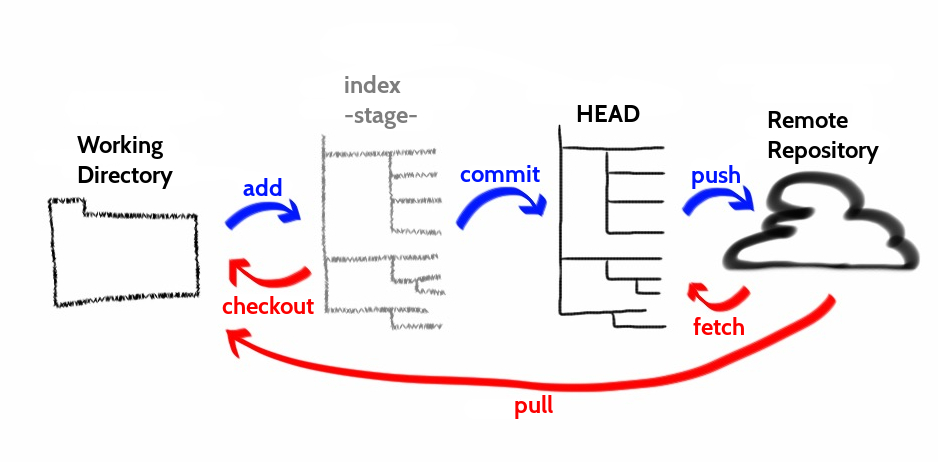
\includegraphics[scale=0.4]{img/git_diagram.jpg} 
\end{center}
\end{figure}

\section{Actualizando directorios: add \& commit}
Para dar una buena idea de c\'omo usar git, vamos a hacer un proyecto simple. En un nuevo repositorio, clonado a nuestro ordenador, vamos a crear un documento nuevo: \textit{gases.py} Ahora, este documento est\'a en nuestro directorio de trabajo o \textbf{w}orking \textbf{d}irectory (WD). Digamos que deseamos pasar este documento de WD a stage. En ese caso, solo escribimos \inlinecode{git add gases.py} en nuestra terminal\footnote{Asegur\'emonos de estar \emph{dentro} del directorio creado con git al clonar el repositorio.} y ya vamos a haber pasado de WD a stage. Esto se puede hacer con cada nuevo documento o archivo, pero si se va a agregar varios simult\'aneamente, la expresi\'on \inlinecode{git add --all} jam\'as puede ser sobrevalorada.\\

Continuando con nuestro peque\~no proyecto, vamos a abrir el documento \textit{gases.py} y vamos a escribir un poco en \'el. Este peque\~no programa nos servir\'a para calcular alguna variable seg\'un el principio de los gases ideales, al prove\'ersele lo dem\'as. Lo primero que debemos hacer es pensar en qu\'e necesitamos en el programa. Evidentemente vamos a requerir:

\begin{itemize}
\item Una funci\'on que le solicite los datos al usuario.
\item Una funci\'on que calcule el resultado de la operaci\'on solicitada.
\item El programa principal con alguna manera de representar los resultados.
\end{itemize}

Entonces, la primera funci\'on se puede ver as\'i:

\begin{Code}
def datos():\\
\hspace*{8mm}print("*** Gases Ideales ***")\\
\hspace*{8mm}print("\ \ \ \ \ P\ V=n\ R\ T")\\
\hspace*{8mm}print("\ \ \ \ \ 1\ 2\ 3\ \ \ 4")\\
\hspace*{8mm}opcion = input("Seleccionar variable a calcularse:\ ")\\
\hspace*{8mm}if opcion >\ 4 or opcion <\ 1:\\
\hspace*{16mm}print("\ \hspace*{-2mm}Opcion invalida!")\\
\hspace*{16mm}return -1, 0, 0, 0\\
\hspace*{8mm}if not (opcion == 1):\\
\hspace*{16mm}presion = float(raw\_input("\ \hspace*{-2mm}Ingresar presion en atmosferas:\ "))\\
\hspace*{8mm}else:\\
\hspace*{16mm}presion = 0\\
\hspace*{8mm}if not (opcion == 2):\\
\hspace*{16mm}volumen = float(raw\_input("\ \hspace*{-2mm}Ingresar volumen en litros:\ "))\\
\hspace*{8mm}else:\\
\hspace*{16mm}volumen = 0\\
\hspace*{8mm}if not (opcion == 3):\\
\hspace*{16mm}moles = float(raw\_input("\ \hspace*{-2mm}Ingresar cantidad de materia en moles:\ "))\\
\hspace*{8mm}else:\\
\hspace*{16mm}moles = 0\\
\hspace*{8mm}if not (opcion == 4):\\
\hspace*{16mm}temperatura = float(raw\_input("\ \hspace*{-2mm}Ingresar temperatura en Kelvin:\ "))\\
\hspace*{8mm}else:\\
\hspace*{16mm}temperatura = 0\\
\hspace*{8mm} return opcion, presion, volumen, moles, temperatura
\end{Code}

Con esto vamos a tener ya la funci\'on que nos captura los datos del usuario y nos los tiene listos para ser calculados. Muchas veces al dejar el proyecto en el que estamos por unos minutos, se nos puede olvidar si hicimos cambios o no, y en d\'onde. Existe un peque\~no comando para determinar si hay cambios y en qu\'e archivos o documentos est\'an. Este es \inlinecode{git status}. Si ejecutamos este comando, sabremos exactamente qu\'e fue alterado. Intent\'emoslo y veamos qu\'e es lo que nos dice git.\\

Ahora que ya entendimos en d\'onde hay cambios es un buen momento para a\~nadir estos al stage a trav\'es de \inlinecode{git add gases.py} Sin embargo, vamos a aprovechar para guardar esto de una manera m\'as profunda, porque realmente esta fue una funci\'on larga. Lo que haremos ahora ser\'a enviar los cambios a HEAD. Eso implica que estos cambios ya merecen un peque\~no mensaje sobre lo que hemos hecho. Es por esto que vamos a proceder de la siguiente manera.\\

Primero vamos a escribir lo siguiente en la terminal: \inlinecode{git commit -m 'Guardando mi primera funci\'on'} Luego vamos a ver c\'omo es que git guarda todo en HEAD. Es un proceso simple que solo muestra algunos de los pasos realizados al hacer \emph{commit} de los cambios. De esta manera git ya tiene algo parecido a una \textit{copia de seguridad} en su directorio reservado. Lo que haremos ahora ser\'a escribir otra funci\'on: la funci\'on que calcula.

\begin{Code}
def calcular(opc, P, V, n, T):\\
\hspace*{8mm}R = 0.0821\\
\hspace*{8mm}if opc == 1:\\
\hspace*{16mm}return "La presion es:\ "\ + str(n * R * T / V)\\
\hspace*{8mm}elif opc == 2:\\
\hspace*{16mm}return "\ \hspace*{-1.5mm}El volumen es:\ "\ + str(n * R * T / P)\\
\hspace*{8mm}elif opc == 3:\\
\hspace*{16mm}return "Los moles son:\ "\ + str(P * V / (R * T))\\
\hspace*{8mm}elif opc == 4:\\
\hspace*{16mm}return "La temperatura es:\ "\ + str(P * V / (R * n))\\
\hspace*{8mm}else:\\
\hspace*{16mm}return "\ \hspace*{-1.5mm}Opcion mal ingresada."
\end{Code}

Perfecto! Con esto ya tenemos una funci\'on que al ingresarle las opciones, nos calcula la variable faltante. Es importante que al terminar de escribirla, nuestro instinto sea el de guardar nuestro trabajo, a\~nadirlo a \textit{stage} y luego a \textit{HEAD}. Para ello vamos a volver a escribir \inlinecode{git add gases.py} y despu\'es de ejecutar ese comando, vamos a escribir el siguiente: \inlinecode{git commit} Si nos damos cuenta, al ejecutar este comando, git abre un editor de texto (que ya deber\'iamos de conocer) para escribir nuestro mensaje all\'i. La ventaja es clara: nos podemos extender, usar caracteres raros, tener varias l\'ineas, etc. Es mucho m\'as c\'omodo escribirlo aqu\'i. Una vez hayamos escrito un mensaje para nuestra nueva funci\'on, vamos a presionar \textbf{Ctrl} + \textbf{X}, luego \textbf{Y} para aceptar los cambios, y finalmente \textbf{Enter} para aceptar el nombre que git le est\'a dando al archivo en el que va nuestro mensaje.\\

Si nos damos cuenta, este proceso de agregar y hacer \emph{commit} a cada funci\'on que terminamos es un proceso repetitivo que debemos ir haciendo peri\'odicamente para no perder nuestros avances. Tambi\'en nos sirve para ir catalogando cada parte del c\'odigo a manera de saber qu\'e se hizo en qu\'e momento y c\'omo. Antes de terminar con nuestro peque\~no programa, vamos a ver c\'omo enviamos cambios a la nube.

\section{Enviar cambios a la nube: push}
Esta parte es quiz\'a la m\'as interesante para muchos. Generalmente git se queda en ir creando copias y versiones de nuestro trabajo en progreso, pero todo cambia y se vuelve mejor cuando lo sincronizamos con la nube. En otras palabras, lo vamos a enviar a un servidor en donde tendremos todo ordenado y listo. Las ventajas de esto son varias:

\begin{itemize}
\item Tendremos una copia de nuestro trabajo aunque algo malo le pase a nuestro ordenador.
\item Muchas otras personas podr\'an colaborar con nosotros en el proyecto que estamos haciendo.
\item Podemos trabajar en el mismo proyecto desde diferentes ordenadores y lugares.
\item Podremos visualizar de mejor manera los cambios realizados por nosotros u otras personas.
\item Todo queda en una plataforma de m\'as f\'acil acceso y m\'as universal: internet.
\end{itemize}

Existen dos maneras de hacer esto. Una es si el repositorio lo creamos en internet y lo clonamos despu\'es a nuestro ordenador. El otro es cuando deseamos enviar cambios de un repositorio creado en nuestro ordenador, a un repositorio remoto ya existente en GitLab o GitHub.\\

Para la primera lo que debemos escribir es lo siguiente: \inlinecode{git push origin master} Lo que queremos decir con esto es que vamos a empujar los cambios, a los que ya hicimos commit, al \emph{origen} del repositorio. Eso de \emph{master} vamos a entenderlo dentro de poco. Al ejecutar este comando, el servicio en l\'inea nos pedir\'a nuestras credenciales y con esto ya podremos subir cambios al repositorio, actualizando as\'i toda la informaci\'on en internet.\\

Para el segundo caso, lo que debemos escribir es de la siguiente manera: \inlinecode{git remote add origin \emph{server}}, en donde \emph{server} es la direcci\'on del repositorio (como la que usamos para clonarlo). Al hacer esto, el servicio tambi\'en nos pedir\'a credenciales. Este m\'etodo se usa muy poco debido a que generalmente es m\'as f\'acil clonar un repositorio y mantenerlo actualizado.\\

Perfecto! Ahora ya sabemos c\'omo mantener conectado todo. Vamos a empujar los cambios de nuestro peque\~no proyecto y a continuaci\'on veremos c\'omo trabajar en colaboraci\'on con m\'as personas de una manera m\'as ordenada.

\section{Ramas}
Una forma de ver el trabajo que hemos realizado es como un hilo al que le vamos agregando nudos; cada nudo es un commit. La idea entonces es ir extendiendo el hilo agreg\'andole un nuevo nudo cada vez. Esta parece ser una manera muy l\'ogica y ordenada de llevar los cambios vamos realiando. Sin embargo, esto nos permite hacer cambios m\'as variados.\\

Supongamos que dos personas comienzan a trabajar en dos partes de un programa. En ese caso ambas van a estar empujando cambios al repositorio, agregando nudos al hilo. El problema es que esto puede llevar a confusiones. De hecho, se vuelve mucho m\'as complicado cuando no se trata de 2 personas, sino de 20. Para estos casos es que vamos a\~nadir un hilo adicional al hilo principal que ya llev\'abamos. Este lo vamos a atar a un nudo en particular (generalmente el \'ultimo que se ha empujado) y en ese ya se puede ir agregando nudos. Si lo consideramos de esta forma, nuestro hilo se va a haber bifurcado en una \emph{rama}. Trabajar cada persona en una rama suele simplificar el desarrollo de un programa o un proyecto, porque se sabe qu\'e cambios son de qui\'en y se puede revisar los avances de una persona exclusivamente. Veamos c\'omo hacer esto ya en nuestro ordenador.\\

\begin{figure}[H]
\begin{center}
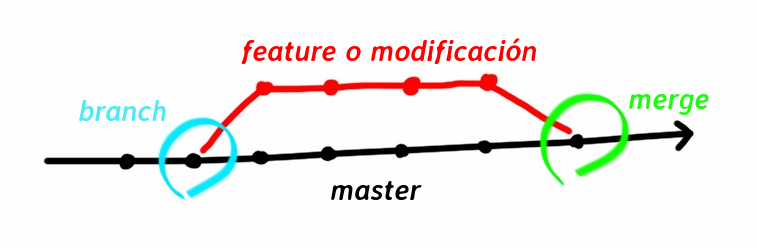
\includegraphics[scale=0.4]{img/branching.jpg} 
\end{center}
\end{figure}

Trabajar con ramas suele ser una tarea sencilla. Si uno se cambia de rama, los documentos y archivos que uno halla al abrir la carpeta del proyecto ser\'an los de \textbf{esa} rama. Esto suena interesante, pero c\'omo se hace en git? Primero necesitar\'iamos crear una rama. Para ello, vamos a escribir \inlinecode{git checkout -b Alternativa} De esta forma habremos creado una rama de nombre \textbf{Alternativa} y nos habremos cambiado a ella. Para notar c\'omo es que las cosas cambian, vamos a terminar nuestro peque\~no programa anterior. Para ello vamos a escribir lo siguiente al final de lo que ya llev\'abamos:

\begin{Code}
o, p, v, n, t = datos()\\
resultado = calcular(o, p, v, n, t)\\
print(resultado)
\end{Code}

Despu\'es de esto, vamos a agregar cambios, hacer commit y subir cambios. Recordando un poco, lo que debemos hacer es: \inlinecode{git add gases.py} Luego seguimos con: \inlinecode{git commit -m 'Terminando el programa'} Y finalmente llegamos a subir todo con: \inlinecode{git push origin Alternativa} Notemos esto \'ultimo! El comando para subir nuestros cambios a la nube ya no es igual. Ahora estamos dici\'endole a git que deseamos empujar a una rama en particular. Esto es muy importante, puesto que si no se hace as\'i, esos cambios no ser\'an subidos en la nueva rama seg\'un GitLab.\\

Ahora que ya hemos subido cambios, vamos a volver a la rama original. Primero vamos a cerrar todos los documentos y archivos que tenemos abiertos. Luego iremos a la Terminal y escribiremos \inlinecode{git checkout master} As\'i habremos regresado a donde est\'abamos. Para comprobar esto, vamos a intentar abrir nuestro programa. Es el mismo que acabamos de hacer? Hay alg\'un cambio? Si hallamos el cambio, felicidades! Esa es la rama original en la que \textit{no} hemos terminado el programa. Vamos a terminar el programa aqu\'i, pero de otra forma, as\'i podemos ir viendo c\'omo es que trabaja git con diferentes ramas.\\

Para hacer un cambio leve y no alterar todo, vamos a terminar nuestro programa de otra manera. Agreguemos el siguiente c\'odigo al final de nuestro programa!

\begin{Code}
o, p, v, n, t = datos()\\
print(calcular(o, p, v, n, t))
\end{Code}

Guardemos esto y luego, con git, vamos a agregarlo a stage, hacer commit y empujar cambios. Al empujar, recordemos que no estamos trabajando en la nueva rama, por lo que el comando ser\'a como antes: \inlinecode{git push origin master} Intentemos revisar en GitLab lo que ha pasado hasta ahora. Es importante notar el cambio de ramas, y las diferencias en el programa. Intentemos ahora cambiar de rama y revisar si los cambios se hicieron bien. Discutamos esto con nuestro compa\~nero de al lado.

\section{Actualizar y fusionar: pull \& merge}
Hasta este momento hemos visto c\'omo ir agregando cosas a nuestro repositorio e ir avanzando. Tambi\'en entendimos que no solo una persona puede trabajar en el respositorio, sino que varias pueden hacerlo a la vez en una sola rama o en varias. El problema ahora ser\'ia: C\'omo tomar en cuenta los cambios de alguien en una versi\'on final? O mejor a\'un! C\'omo actualizo yo mi repositorio local (el que tenego en mi ordenador) con los cambios de alguien m\'as? Pues para eso hay otros comandos que nos pueden servir.\\

Supongamos que estamos trabajando con alguien m\'as. Nosotros comenzamos el repositorio, empujamos algo varias veces y luego dejamos el trabajo para seguir al d\'ia siguiente. Sin embargo, nuestro compa\~nero hace algunos otros cambios en la misma rama durante la noche y los empuja al repositorio. Al d\'ia siguiente, los cambios nuestros y de nuestro compa\~nero est\'an en el repositorio en la nube, pero no en nuestro repositorio local. Lo que nos toca hacer es actualizar nuestro repositorio local. Para ello vamos a utilizar el siguiente comando: \inlinecode{git pull} Solamente eso! Al ejecutar este comando vamos a haber actualizado nuestro ordenador con todos los cambios que se hallan en la nube.\\

Pero qu\'e pasa cuando ambos trabajan en el mismo repositorio, pero no en la misma rama? Es una buena pr\'actica que cada uno trabaje independientemente en una rama para lograr ordenar mejor los cambios. Sin embargo, habr\'an momentos en que vamos a querer tener una versi\'on final que comprenda los cambios y avances empujados por todos. En este caso, lo que hacemos es ir a la rama sobre la que deseamos trabajar y vamos a fusionar otra rama sobre esta. Regresando al ejemplo anterior, estamos trabajando con un compa\~nero que empuj\'o sus cambios a su rama \emph{Compa} hace unos minutos. Ahora deseamos que esos cambios lleguen a la rama \emph{master}, puesto que con ellos terminamos nuestro proyecto. Para ello, primero nos vamos a la rama \emph{master} con el comando \inlinecode{git checkout master} Luego procedemos a fusionar la rama \emph{Compa} sobre la rama \emph{master}. Recordems que la rama debe de existir en la nube, no exclusivamente en nuestro repositorio. Para ello ejecutamos \inlinecode{git merge origin/Compa}. Luego empujamos cambios de manera normal y todo listo! Hemos fusionado la rama.\\

Claro, no deben de haber conflictos, como cuando los dos escriben en el mismo archivo en la misma l\'inea, o que hayan hecho cambios a la vez, etc. De existir estos conflictos, git intentar\'a advertirnos que hay l\'ineas con dos versiones diferentes del c\'odigo, y nos tocar\'a escoger qu\'e cambios dejar en el repositorio.

\section{Reemplazar cambios locales: checkout, fetch \& reset}
Un caso que se puede dar y a pesar de ser desagradable es muy com\'un, es que hagamos un cambio en un archivo, lo guardemos y luego nos damos cuenta de que no dese\'abamos guardar eso. Para esos casos, podr\'iamos simplemente descargar la \'ultima versi\'on del repositorio, borrando as\'i los cambios que hemos hecho. Para hacer eso, el comando que aplicamos es el siguiente: \inlinecode{git checkout -- nombre\_del\_archivo.txt} Si ya hab\'iamos agregado alg\'un archivo con \textit{add} o hab\'iamos creado algo, no debemos preocuparnos; esto no se ver\'a afectado.\\

Por otra parte, si deseamos ignorar todos los cambios hechos y solo descargar la \'ultima versi\'on de un proyecto almacenada en nuestro repositorio, podemos hacerlo con \inlinecode{git fetch origin} Es conveniente advertir que si hacemos esto y hab\'iamos realizado alg\'un cambio importante que dese\'abamos conservar, lo vamos a perder por siempre. Por esta raz\'on es importante saber bien qu\'e se est\'a haciendo con \textit{status}.\\

La mayor parte de estos comandos y estas herramientas son dif\'iciles de aprender a menos de que uno las vaya usando poco a poco. Es despu\'es de varios aciertos y errores que vamos a ir entendiendo c\'omo se utiliza cada cosa. Durante el taller podemos ir haciendo uso de algunas de estas herramientas, pero tenemos que tomar en cuenta que no se nos ayudar\'a m\'as; ya deber\'iamos de dominar esto. Para ello vamos a comenzar con un proyecto en particular y vamos a irlo desarrollando poco a poco entre todos los presentes.

\section{Proyecto}
El proyecto en el que vamos a trabajar ya est\'a creado en un repositorio de GitLab. Por esta raz\'on solo vamos a clonar el proyecto de esta direcci\'on: \href{https://gitlab.com/zronyj/TC3Q\_ej.git}{https://gitlab.com/zronyj/TC3Q\_ej.git} Al ya haber clonado el proyecto, entraremos en la carpeta correspondiente y comenzaremos a trabajar. Lo primero que haremos ser\'a entrar a la carpeta \textbf{Users} y crear un documento de texto que contenga nuestro nombre completo, nuestra fecha de cumplea\~nos y si somos estudiantes, catedr\'aticos o investigadores en una l\'inea diferente cada cosa. Luego vamos a guardar este documento bajo el siguiente nombre: \emph{apellidoNombre.txt} en donde el apellido y el nombre son \textbf{tu} apellido y \textbf{tu} nombre. Finalmente nos saldremos de la carpeta \textbf{Users} y quedaremos listos para el siguiente paso.\\

En los d\'ias anteriores hemos visto algunos principios b\'aiscos para programar rutinas o peque\~nos programas. Hoy vamos a comenzar con uno que nos va a servir para ejemplificar el uso de git. Nos vamos a dividir en 4 grupos y vamos a intentar hacer 4 programas sencillos; uno por grupo. De esta manera vamos a entender mejor c\'omo es que funciona git. Los programas son:

\begin{enumerate}
\item \textbf{Fisicoqu\'imica:} peque\~no programa al que le demos la entalp\'ia, entrop\'ia y temperatura (en Kelvin) de los productos y de los reactivos de una reacci\'on, y este nos muestre las diferencias calculadas entre reactivos y productos para entalp\'ia $\Delta H$, entrop\'ia $\Delta S$ y energ\'ia libre de Gibbs $\Delta G$. Como dato importante, esta f\'ormula puede ser \'util: $\Delta G = \Delta H - T \cdot \Delta S$ Y para calcular diferencias, solo basta con una simple resta: $\Delta H = H_{prods} - H_{reacts}$
\item \textbf{An\'alisis:} peque\~no programa que calcula el pH de una soluci\'on de \'acido ac\'etico solo introduci\'endole el volumen de \'acido ac\'etico agregado $V_{HAc}$, la concentraci\'on del mismo $\left[ HAc \right]$ y el volumen de agua sobre el que se est\'a agregando $V_{H_2 O}$. Como datos importantes, este equilibrio viene dado por: $K = \frac{\left[ H^+ \right] \left[ Ac^- \right]}{\left[ HAc \right]}$ Para calcular concentraciones a vol\'umenes nuevos, se hace esto: $\left[ HAc \right]_{nueva} = \frac{\left[ HAc \right] \cdot V_{HAc}}{V_{H_2 O} + V_{HAc}}$ Y el pH se calcula de esta manera: $pH = - \log_{10} \left( \left[ H^+ \right] \right)$ La constante es $K = 1.77 \cdot 10^{-5}$
\item \textbf{Org\'anica:} peque\~no programa que calcula la cantidad de insaturaciones en una mol\'ecula, dada la f\'ormula. La mol\'ecula puede tener hal\'ogenos, ox\'igeno y/o nitr\'ogeno. Como dato importante, la f\'ormula para hacer esto se ve de la siguiente manera: $IDH = C - \frac{H}{2} + \frac{N}{2} + 1$ en donde $C$ es el n\'umero de \textbf{c}arbonos, $H$ es el n\'umero de \textbf{h}idr\'ogenos o \textbf{h}al\'ogenos y $N$ es el n\'umero de \textbf{n}itr\'ogenos. El programa tiene que aceptar el ingreso de los elementos uno por uno.
\item \textbf{Inorg\'anica:} peque\~no programa que calcula la densidad de un metal basado en el volumen de la unidad cristalina m\'as peque\~na. Para ello se indica si la unidad es c\'ubica simple (\emph{PCC}), c\'ubica centrada en el cuerpo (\emph{BCC}) o c\'ubica centrada en las caras (\emph{FCC}). Como dato importante se ha de mencionar que la f\'ormula para calcular el volumen de la PCC es: $V_{PCC} = \left( 2 r \right)^3$, la f\'ormula para calcular la BCC es: $V_{BCC} = \left( \frac{4 \sqrt{3} r}{3} \right)^3$ y la f\'ormula para calcular FCC es $V_{FCC} = \left( 2 \sqrt{2} r \right)^3$. Claro, $r$ es el radio at\'omico del metal del que deseamos calcular. En la PCC hay 1 \'atomo del metal en cuesti\'on. En la BCC hay 2 \'atomos. Y en la FCC hay 4 \'atomos. Y claro, la densidad es siempre: $\rho = \frac{m}{V}$
\end{enumerate}

No nos vayamos a complicar la vida haciendo estos programas, la idea es mantener la simplicidad. 

\section{Comentarios finales}
Felicidades, completaste la s\'eptima sesi\'on del $TC^3 Q$. En el futuro, si deseas hacer alg\'un trabajo de desarrollo de aplicaciones, investigaci\'on en general, o dejar registro del progreso de un proyecto, es conveniente que utilices este tipo de herramienta para poder llevar registro de todos los cambios y versiones. M\'as adelante en el taller, puedes hacer uso de git para ir almacenando los cambios y avances que vas realizando.\\

Si deseas aprender m\'as sobre git, puedes buscar otros tutoriales en internet. Sin embargo, para fines de investigaci\'on es recomendable que veas qu\'e es lo que puede hacer \href{http://figshare.org/}{FigShare} con el trabajo que ya hemos desarrollado en git. Son muchas m\'as utilidades las que se les ha dado a esta herramienta. Busca y piensa qu\'e podr\'ias hacer con ella aunque no se tratara de ir llevando control de los cambios en un proyecto.\\

En la pr\'oxima sesi\'on vamos a profundizar un poco m\'as sobre c\'alculo de algunas propiedades moleculares y sobre los formatos en los que almacenamos las mol\'eculas. Recuerda resolver todas tus dudas antes de continuar. Fuera de eso, felicidades nuevamente! Lograste terminar una sesi\'on m\'as!

\subsection{Glosario de comandos sencillos}
\begin{small}
\begin{itemize}
\item \textbf{git config}: configura git con tu nombre, tu direcci\'on de correo y tu editor de texto preferido.
\item \textbf{git init}: inicia un nuevo proyecto en git de manera local; un nuevo repositorio.
\item \textbf{git clone}: descarga los contenidos de un repositorio ya existente a tu ordenador y los deja listos para poder trabajar con ellos.
\item \textbf{git status}: revisa el estado actual de los archivos en el repositorio en comparaci\'on al \'ultimo commit.
\item \textbf{git diff}: muestra claramente las diferencias entre el estado actual de los archivos en el repositorio con respecto al \'ultimo commit. Muestra las diferencias l\'inea por l\'inea.
\item \textbf{.gitignore}: archivo que contiene el listado de todos los archivos del proyecto que deben ser ignorados por git.
\item \textbf{git commit}: guarda los cambios realizados a los archivos como una revisi\'on. Crea un registro y un \emph{id} que identifica a esa revisi\'on.
\item \textbf{git push}: empuja (sube) los commits locales a GitHub.
\item \textbf{git pull}: jala (descarga) los archivos del proyecto en GitHub, actualizando el estado de estos en nuestro ordenador.
\item \textbf{git log}: muestra toda la actividad de commits que ha habido en un repositorio/proyecto.
\item \textbf{git branch}: muestra a todas las ramas existentes o, si se le agrega un nombre despu\'es del comando, se crea una rama nueva en el proyecto.
\item \textbf{git merge}: une a una rama existente con otra rama que se debe de especificar como argumento del comando.
\item \textbf{git checkout}: si como argumento se agrega el nombre de una rama, se habr\'a trasladado a esa rama. Si como argumento se agrega el \emph{id} de un commit o la distancia de la cabeza a un commit con \inlinecode{HEAD$\sim$\#}, entonces nos situaremos en el commit seleccionado y podremos ver el estado del proyecto en ese momento.
\end{itemize}
\end{small}

\section*{Licencia}

\noindent 
\includegraphics{img/cc_big.png}

\noindent Taller de Qu\'imica Computacional Aplicada by \href{http://github.com/zronyj/TC3Q}{Rony J. Letona} is licensed under a \href{http://creativecommons.org/licenses/by-sa/4.0/}{Creative Commons Attribution-ShareAlike 4.0 International License}.
Based on a work at \url{http://github.com/swcarpentry/bc} and \url{http://rogerdudler.github.io/git-guide/index.es.html}.

\end{document}
